\documentclass[border=3pt]{standalone}
% Preâmbulo compartilhado pelos diagramas TikZ da aula 8 de Navegação (Implementação do RRT)
\usepackage[T1]{fontenc}
\usepackage[utf8]{inputenc}
\usepackage{lmodern}
\usepackage{amsmath}
\usepackage{xcolor}
\usepackage{tikz}
\usetikzlibrary{arrows.meta,angles,quotes,decorations.pathmorphing,decorations.pathreplacing,calc,
                positioning,shapes.geometric,shapes.misc,backgrounds,fit,
                math}

% Paleta (mesma dos SVGs originais)
\definecolor{dblue}{HTML}{2A5B8C}
\definecolor{dorange}{HTML}{B3541E}
\definecolor{dgreen}{HTML}{4A7C59}
\definecolor{dred}{HTML}{9C4B4B}
\definecolor{dcream}{HTML}{F4F1EA}
\definecolor{dshade}{HTML}{DDD7C9}

% Função gaussiana (não normalizada por padrão de escala visual)
\pgfmathdeclarefunction{gauss}{3}{%
  \pgfmathparse{1/(#3*sqrt(2*pi))*exp(-((#1-#2)^2)/(2*#3^2))}%
}

% Estilos comuns (prefixo d... para não colidir com chaves internas do pgf)
\tikzset{
  >={Stealth[length=2mm]},
  dguide/.style={gray!55, dashed, line width=0.4pt},
  daxis/.style={gray!60, line width=0.7pt, ->},
  dbody/.style={fill=black!3, draw=black!80, line width=1pt},
  dacc/.style={draw=dblue, line width=1pt},
  dlbl/.style={black!55, font=\small},
  dsub/.style={black!45, font=\footnotesize},
  dstate/.style={circle, draw=black!80, fill=dcream, line width=1pt,
                 minimum size=17mm, font=\large, inner sep=1pt},
  dobs/.style={circle, draw=black!80, fill=dshade, line width=1pt,
               minimum size=14mm, font=\large, inner sep=1pt},
  dbox/.style={rounded corners=2pt, draw=black!80, fill=dcream, line width=1pt,
               align=center, inner sep=6pt},
  dop/.style={circle, draw=black!80, fill=white, line width=1pt,
              minimum size=6mm, inner sep=0pt, font=\small},
  dtrans/.style={->, dblue, line width=1pt},
  dmeas/.style={->, dorange, line width=1pt},
  dcurve/.style={line width=1pt, dblue},
  dcurveb/.style={line width=1.4pt, dorange},
}

\begin{document}
\hyphenpenalty=10000 \exhyphenpenalty=10000 \tolerance=9999 \emergencystretch=3em
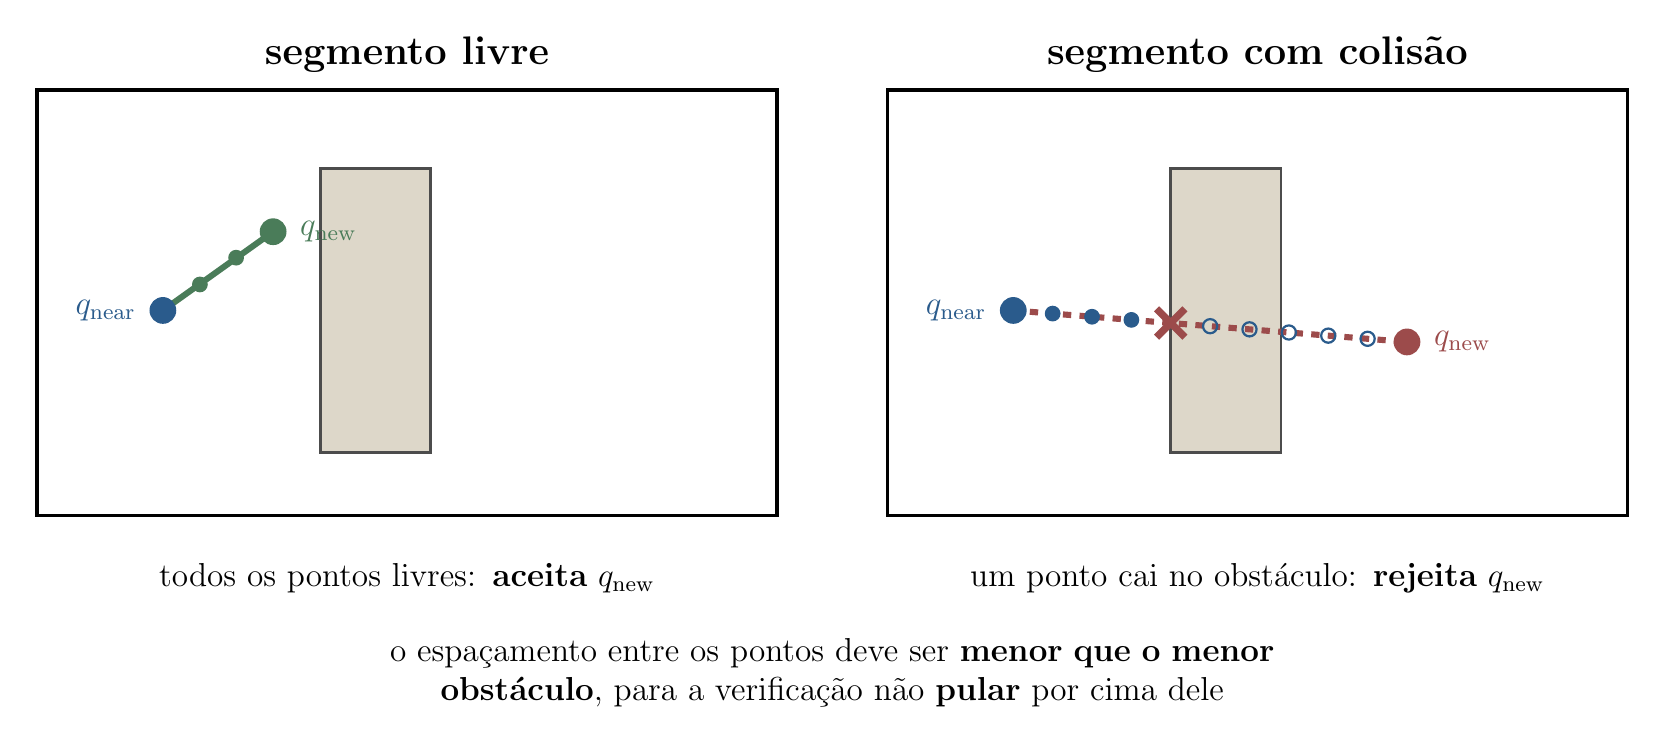
\begin{tikzpicture}[x=1cm,y=1cm]
\draw[line width=1.2pt, fill=white] (0.00,0) rectangle (9.40,5.4);
\draw[line width=1pt, draw=black!70, fill=dshade] (3.60,0.80) rectangle (5.00,4.40);
\draw[dgreen, line width=2.2pt] (1.60,2.60) -- (3.00,3.60);
\fill[dgreen] (1.60,2.60) circle (0.1);
\fill[dgreen] (2.07,2.93) circle (0.1);
\fill[dgreen] (2.53,3.27) circle (0.1);
\fill[dgreen] (3.00,3.60) circle (0.1);
\fill[dblue] (1.60,2.60) circle (0.17); \node[font=\large\bfseries, text=dblue, anchor=east] at (1.38,2.60) {$q_{\mathrm{near}}$};
\fill[dgreen] (3.00,3.60) circle (0.17); \node[font=\large\bfseries, text=dgreen, anchor=west] at (3.22,3.60) {$q_{\mathrm{new}}$};
\node[font=\Large\bfseries, anchor=south] at (4.70,5.5) {segmento livre};
\node[font=\large, text width=9.4cm, align=center] at (4.70,-0.8) {todos os pontos livres: \textbf{aceita} $q_{\mathrm{new}}$};
\draw[line width=1.2pt, fill=white] (10.80,0) rectangle (20.20,5.4);
\draw[line width=1pt, draw=black!70, fill=dshade] (14.40,0.80) rectangle (15.80,4.40);
\draw[dred, line width=2.2pt, dashed] (12.40,2.60) -- (17.40,2.20);
\fill[dblue] (12.40,2.60) circle (0.1);
\fill[dblue] (12.90,2.56) circle (0.1);
\fill[dblue] (13.40,2.52) circle (0.1);
\fill[dblue] (13.90,2.48) circle (0.1);
\draw[dred, line width=2.6pt] (14.40,2.44) -- ++(0.18,0.18) (14.40,2.44) -- ++(0.18,-0.18) (14.40,2.44) -- ++(-0.18,0.18) (14.40,2.44) -- ++(-0.18,-0.18);
\draw[dblue, line width=0.8pt] (14.90,2.40) circle (0.09);
\draw[dblue, line width=0.8pt] (15.40,2.36) circle (0.09);
\draw[dblue, line width=0.8pt] (15.90,2.32) circle (0.09);
\draw[dblue, line width=0.8pt] (16.40,2.28) circle (0.09);
\draw[dblue, line width=0.8pt] (16.90,2.24) circle (0.09);
\draw[dblue, line width=0.8pt] (17.40,2.20) circle (0.09);
\fill[dblue] (12.40,2.60) circle (0.17); \node[font=\large\bfseries, text=dblue, anchor=east] at (12.18,2.60) {$q_{\mathrm{near}}$};
\fill[dred] (17.40,2.20) circle (0.17); \node[font=\large\bfseries, text=dred, anchor=west] at (17.62,2.20) {$q_{\mathrm{new}}$};
\node[font=\Large\bfseries, anchor=south] at (15.50,5.5) {segmento com colisão};
\node[font=\large, text width=9.4cm, align=center] at (15.50,-0.8) {um ponto cai no obstáculo: \textbf{rejeita} $q_{\mathrm{new}}$};
\node[font=\large, text width=20cm, align=center] at (10.1,-2.0) {o espaçamento entre os pontos deve ser \textbf{menor que o menor obstáculo}, para a verificação não \textbf{pular} por cima dele};
\end{tikzpicture}
\end{document}
